\documentclass[12pt,a4paper,titlepage]{article}
\usepackage[utf8x]{inputenc}
\usepackage[francais]{babel}
\usepackage[T1]{fontenc}
\usepackage{amsmath}
\usepackage{amsfonts}
\usepackage{amssymb}
\usepackage{makeidx}
\usepackage{graphicx}
\usepackage{hyperref}
\usepackage[left=2cm,right=2cm,top=2cm,bottom=2cm]{geometry}

\hypersetup{colorlinks=true, linkcolor=blue, citecolor=blue, filecolor=blue, urlcolor=blue, pdftitle=Documentation administrateur ZenFusion, pdfauthor=Sébastien Bodrero Raphaël Doursenaud, pdfsubject=, pdfkeywords=}

\author{Sébastien \textsc{Bodrero}, Raphaël \textsc{Doursenaud}}

\title{ZenFusion™ pour Google Apps™ : Documentation Administrateur}

\date{\today}

\begin{document}
	
\begin{titlepage}

	\begin{center}

	
\includegraphics{ZenFusion}
	
	\end{center}
	

\end{titlepage}
		
	
	\section{Installation}
	
		\subsection{Pré-requis}
		
		\begin{itemize}
			\item Dolibarr 3.0 et supérieur
			\item PHP 5.0.0 ou supérieur
			\item BDD MySQL
			\item les extensions PHP suivantes :
			\begin{itemize}
				\item \href{http://pecl.php.net/package/oauth}{OAuth}
				\item PCRE
				\item simpleXML
			\end{itemize} 
		\end{itemize}
		
		\paragraph{}
			\textbf{OAuth}\footnote{OAuth est un protocole libre, créé par Blaine Cook et Chris Messina qui permet l'authentification à une API sécurisée d'une façon simple et standard depuis son bureau ou une application web. Pour les développeurs d'une application accédant à une API, OAuth est une façon de publier et d'interagir avec des données protégées. Pour les développeurs fournissant une API, OAuth permet de donner accès aux données tout en protégeant le pseudo et mot de passe des utilisateurs. Source \url{http://fr.wikipedia.org/wiki/OAuth}} est le système d'authentification choisi pour garantir la sécurité et l'intégrité des transactions entre \emph{Dolibarr} et \emph{Google Apps}. Ce dernier se présente sous la forme d'une extension PHP de type \emph{\href{pecl.php.net}{PECL}}.
			
			\bigskip
			
			Exemple d'installation sur systèmes Debian et dérivés :
			
			\begin{verbatim}
				# apt-get install php-pear
				# apt-get install libpcre3-dev
				# pecl install oauth
			\end{verbatim}
			
			% À vérifier dès que la VM est installée
			Éditer \emph{php.ini} et ajouter :
			\begin{verbatim}
			extension=oauth.so
			\end{verbatim}
		
	\subsection{Installation de ZenFusion}
	
		\paragraph{}
		ZenFusion se compose de deux modules interdépendants : 
		
		\begin{itemize}
		\item ZenFusion OAuth : Gère l'authentification et assure les requêtes de façon sécurisée
		\item ZenFusion Contacts : Intégration des Tiers et Contacts avec Google™ Contacts.
		\end{itemize}
		
		\paragraph{}
		Décompresser l'archive \textbf{ZenFusion-\textit{version}.tgz} à la racine de votre d'installation \emph{Dolibarr}.

		\section{Activation des modules}
		
		\begin{figure}[h]
			\centering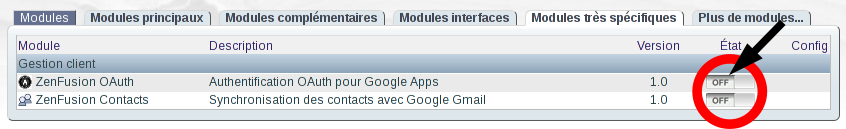
\includegraphics[scale=0.55]{activation1}
			\caption{Modules désactivés}
			\label{fig:act}
		\end{figure}	
	
		\begin{itemize}
			\item Se connecter en tant qu'administrateur
			\item Dans \textbf{Configuration⇒Modules⇒Modules très spécifiques}, activer les modules :
				\begin{itemize}
					\item ZenFusion OAuth
					\item ZenFusion Contacts
				\end{itemize}			
		\end{itemize}
	
	\section{Outils}
		
		\begin{figure}[h]
			\centering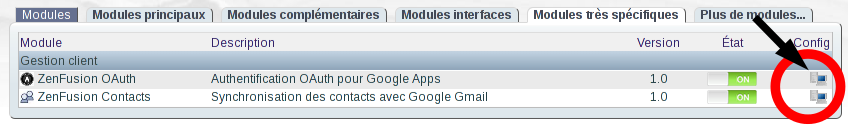
\includegraphics[scale=0.55]{conf1}
			\caption{Outils}
			\label{fig:conf}
		\end{figure}		
		
		\paragraph{}
		L'icône 
\includegraphics{setup} des modules permet d'accéder aux outils.
		\emph{Notez que tous les modules donnent accès au même jeu d'outils.}
		
		\subsection{Statistiques}
		
		\paragraph{}
		Les \emph{statistiques} permettent à l'administrateur de connaître le nombre de contacts synchronisés par utilisateur.
		
		\subsection{Assistance \textit{(Optionnel)}}
		
		\paragraph{}
		Cet onglet n'apparaît que si vous avez souscrit à un contrat d'assistance.		
		
		\paragraph{}
		En fonction de votre contrat vous pouvez bénéficier d'une assistance utilisateur.
		Si tel est votre cas, cliquez sur l'onglet \emph{Assistance} puis sur le lien afin d'entrer en contact avec notre équipe de techniciens.
		
		% TODO illustration !
	
		\subsection{À propos}
		\paragraph{}
		Présente les informations suivantes :
		
		\begin{itemize}
			\item Version
			\item Éditeur
			\item Licence
			\item Crédits	
		\end{itemize}
	
	\section{FAQ}
		\paragraph{}
		Veuillez vérifier les points suivants à l'origine des principales erreurs du module \textbf{ZenFusion} :
		 \begin{itemize}
		 \item Droits de lecture et d'exécution sur les dossiers du module \textbf{ZenFusion} 
		 \item Présence du module \emph{OAuth} sur le serveur. Pensez à regarder votre PHPinfo !
		 \item Extension oauth.so active dans votre fichier \emph{php.ini}
		 \item Extensions PHP \emph{PCRE} et \emph{simpleXML} présentes sur le serveur
		 \item Votre serveur doit être connecté à \emph{Internet} 
		 \item Adresses email \emph{Google Gmail}
		 \item L'adresse email de votre utilisateur doit être renseignée dans sa fiche
		 \item L'utilisateur doit autoriser l'application à acceder aux informatios de son compte \emph{Google Gmail}
		\end{itemize}
\end{document}
